\section{Motores de combustión Interna}

Los motores de combustión interna dieron un impulso a la actividad humana
desde los años 1860, donde su uso comercial comenzó a popularizarse.
%
La función de estos dispositivos es la de convertir la energía potencial del
fluido de trabajo, una mezcla de aire\-combustible, en trabajo mecánico por
medio de una combustión controlada dentro de una cámara de combustión.
%
Los primeros ejemplares comerciales eran voluminosos, costosos, altamente
ineficientes y de baja potencia, con valores de rendimiento cercano al 5\% y
potencias de hasta 6 HP.

Un paso importante hacia los motores actuales fue el desarrollo del ciclo Otto,
propuesto por Nicolaus A. Otto y Eugen Langen, cuyo primer prototipo se puso en
marcha en el año 1876.
%
Otto propuso un motor alternativo con cuatro carreras de pistón: admisión,
compresión, expansión y escape; este prototipo lograba la misma potencia y
mayor eficiencia que los motores de la época con menos de la mitad del peso y
volumen.
%
En la figura \ref{fig:otto1909} se ve un motor de ciclo otto fabricado por
\emph{Otto Gas Engines Works} 1909 en Filadelfia-EEUU, según la revista
\emph{Gas Engine
Magazine}\footnote{\url{https://www.gasenginemagazine.com/gas-engines/1909-5-hp-otto-special-electric/}}
\footnote{ \url{https://www.youtube.com/watch?v=LPSWfg0Y3Hs} } \footnote{
    \url{https://www.youtube.com/watch?v=0d0WZ0H56_U} }, este motor
originalmente estaba directamente acoplado a una bomba triplex de agua que era
parte de un sistema de irrigación a un club de campo de Delaware.

\begin{figure}
    \centering
    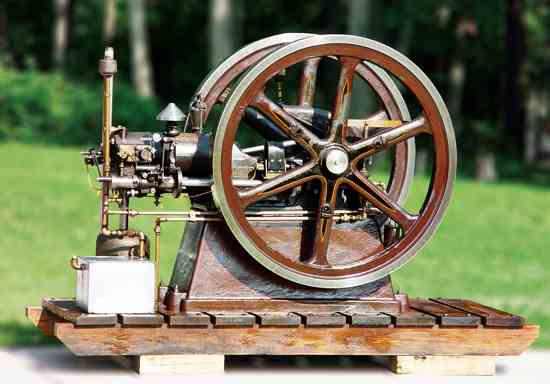
\includegraphics[width=.5\textwidth]{otto_1909.jpg}
    \caption{Motor 1909 5HP Otto Special Electric Lighting de Wayne Grenning}\label{fig:otto1909}
% https://www.gasenginemagazine.com/gas-engines/1909-5-hp-otto-special-electric/
\end{figure}

Los motores han continuado su desarrollo desde entonces, mejorando materiales,
combustibles y procesos de manufactura entre otros.
%
Además, en las últimas décadas se ha hecho foco en disminuir el consumo de
combustible y las emisiones de gases contaminantes como las de $CO_2$ y $NO_x$,
el nivel de ruido, costo de manufactura, tamaño, etc.

%%%%%%%%%%%%%%%%%%%%%%%%%%%%%%%%%%%%%%%%%%%%%%%%%%%%%%%%%%%%%%%%%%%%%%%%%%%%%%%
\subsection{Ciclo operativo}
%
Los motores reciprocantes de combustión interna existen de 2 o 4 tiempos, esto
hace referencia a la cantidad de carreras del pistón necesarias para producir
una carrera de expansión (o potencia), las cuatro carreras son: admisión,
compresión, expansión y escape; ilustradas en la figura \ref{fig:4tiempos}.
%
En el movimiento del pistón se pueden identificar dos posiciones de interés:
punto muerto superior (PMS) y punto muerto inferior (PMI), en el PMS se tiene
el volumen mínimo atrapado en el cilindro, en el PMI, se tiene el volumen
máximo del cilindro y la diferencia entre el volumen en el PMS y el PMI es el
volumen desplazado $V_D$, \ref{fig:pms_pmi}.

\begin{figure}
    \centering
    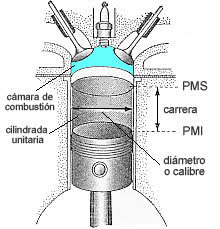
\includegraphics[width=0.4\textwidth]{pms_pmi.jpg}
    \caption{PMS y PMI}\label{fig:pms_pmi}
    % https://www.istockphoto.com/es/vector/motor-di%C3%A9sel-de-cuatro-tiempos-gm586705100-100702521
\end{figure}

De manera simplificada, asumiendo que la apertura y cierre de las válvulas de
admisión y escape son instantáneas, el ciclo de cuatro tiempos de un motor de
encendido por chispa se puede describir como:
%
\begin{itemize}
%
    \item Admisión, el pistón se mueve desde el PMS hasta el PMI con la válvula
        de admisión abierta y la de escape cerrada, esto hace que ingrese una
        masa de aire-combustible al cilindro.
%
    \item Compresión, el pistón se mueve desde el PMI hacia el PMS con las
        válvulas de admisión y escape cerradas, esta reducción del volumen
        comprime y calienta los gases en el interior del cilindro.
        %
        Es durante la carrera de compresión que se enciende la mezcla.
%
    \item Expansión, la combustión produce un aumento de presión y temperatura
        en el cilindro, la carrera de expansión parte del PMS hacia el PMI,
        aprovechando la expansión en volumen de los productos de la combustión
        que producen trabajo sobre la cara del pistón, el cual lo transfiere al
        cigüeñal.
%
    \item Escape, luego de la carrera de expansión, en el PMI se abre la
        válvula de escape y el movimiento del pistón hacia el PMS hace un
        barrido de los gases quemados.
%
\end{itemize}

\begin{figure}
    \centering
    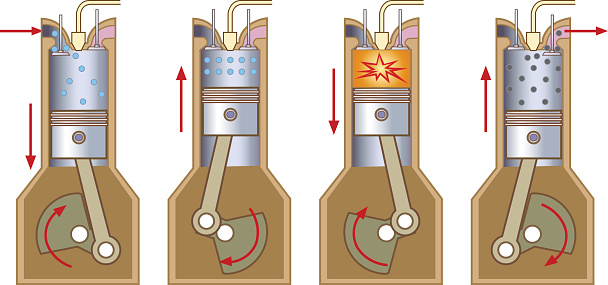
\includegraphics[width=0.7\textwidth]{4stroke.jpg}
    \caption{Ciclo de cuatro tiempos}\label{fig:4tiempos}
    % https://www.istockphoto.com/es/vector/motor-di%C3%A9sel-de-cuatro-tiempos-gm586705100-100702521
\end{figure}

%%%%%%%%%%%%%%%%%%%%%%%%%%%%%%%%%%%%%%%%%%%%%%%%%%%%%%%%%%%%%%%%%%%%%%%%%%%%%%%

\subsection{Combustión}
%
La combustión es un proceso en el que se libera la energía química del
combustible, la geometría de un motor de combustión interna permite aprovechar
el aumento de presión y temperatura que ocurre en la cámara para convertir esta
energía en trabajo mecánico.
%

Los modelos ideales de ciclos operativos se pueden clasificar según el proceso
de combustión en,
%
\begin{enumerate}
        %
    \item a volumen constante
        %
    \item a presión constante
        %
    \item a presión limitada (parte a volumen constante y parte a
        presión constante)
        %
\end{enumerate}

En un motor de encendido por chispa, se tiene una mezcla de aire-combustible en
la cámara de combustión, dependiendo del tipo de motor, la mezcla se puede
formar en el conducto de admisión, inyectando combustible en algún punto del
sistema o se puede producir la mezcla en la cámara por la inyección directa de
combustible.
%
En un motor de encendido por compresión, la mezcla combustible se forma en la
cámara de combustión, luego de la inyección directa del combustible.

\begin{figure}
    \centering
    \begin{subfigure}{0.4\textwidth}
        \centering
        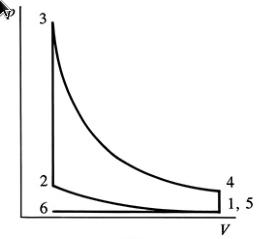
\includegraphics[width=\textwidth]{combustion_vol_cte.jpg}
        \caption{Combustión a Volumen Constante}
    \end{subfigure}
    \hfill
    \begin{subfigure}{0.4\textwidth}
        \centering
        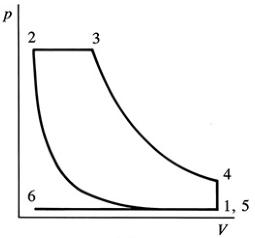
\includegraphics[width=\textwidth]{combustion_presion_cte.jpg}
        \caption{Combustión a Presión Constante}
    \end{subfigure}
    \hfill
    \begin{subfigure}{0.4\textwidth}
        \centering
        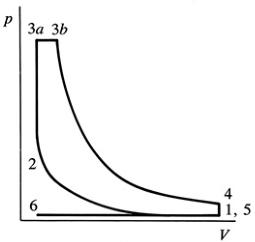
\includegraphics[width=\textwidth]{combustion_presion_limitada.jpg}
        \caption{Combustión a Presión Limitada}
    \end{subfigure}
    \caption{Diagramas P-V para ciclos ideales\parencite{heywood}}\label{fig:ciclos_ideales}
\end{figure}

El MRCVC es un motor de combustión interna encendido por chispa en el que,
gracias al a geometría del mismo, gran parte de la combustión ocurre a volumen
constante, como se puede apreciar en la figura \ref{fig:vol_constante}.
%
En este trabajo no se estudia el proceso de combustión del MRCVC, sin embargo
se describe el motivo por el que la combustión a volumen constante es más
eficiente que la combustión a presión constante.

En \parencite{heywood} se hace un análisis de los modelos operativos de gas
ideal, en los cuales se asume que
% El mayor rendimiento de la combustión a volumen constante se puede ver
% analizando los modelos ideales de ciclos operativos \parencite{heywood},
el fluido de trabajo es gas ideal, con $C_v$ y $C_p$ constantes.
%
Se pueden analizar los 3 casos de combustión: volumen constante, a presión
constante o a presión limitada, obteniendo expresiones para el rendimiento de
conversión de combustible \ref{eq:rendimiento_p_lim} y de $imep$ en función de
la presión mínima del ciclo $p_1$ \ref{eq:imep_p1} y máxima $p_3$
\ref{eq:imep_p3}.

La combustión a volumen constante a presión constante son casos extremos de la
combustión a presión limitada, por lo que se puede utilizar  el rendimiento de
conversión de combustible para el ciclo de presión limitada es para comparar
entre ambos.

\begin{align}
    \label{eq:rendimiento_p_lim}
    %
    \eta_{f,i} &= 1 - \frac{1}{r_c^{\gamma - 1}} \left[ \frac{\alpha \beta^\gamma-1}{\alpha \gamma (\beta-1)+\alpha-1} \right]\\
    \alpha &= \frac{P_3}{P_2}\\
    \beta &= \frac{V_{3b}}{V_{3a}}
    %
\end{align}

\begin{equation}
    \label{eq:imep_p1}
    \frac{imep}{p_1} = \frac{Q^*}{c_v T_1 (\gamma-1)} \left( \frac{r_c}{r_c-1} \right) \eta_{f,i}
    %
\end{equation}

\begin{equation}
    \label{eq:imep_p3}
    \frac{imep}{p_3} = \frac{1}{\alpha r_c^\gamma} \left( \frac{Q^*}{c_v T_1}
    \right) \left(\frac{1}{\gamma-1} \right) \left( \frac{r_c}{r_c-1} \right)
    \eta_{f,i}
    %
\end{equation}

En el caso en que  $\alpha=1 \rightarrow P_3=P_2$ y se tiene el ciclo de
combustión a presión constante, en el caso en que $\beta=1 \rightarrow
V_{3a}=V_{3b}$ y se tiene el ciclo de combustión a volumen constante, como se
ve en la figura \ref{fig:ciclos_ideales}.

Graficando la ecuación \ref{eq:rendimiento_p_lim} en función de la relación de
compresión $r_c$ (figura \ref{fig:rendimientos}), para distintos valores se ve
que a igual relación de compresión, el ciclo a volumen constante presenta mayor
rendimiento de conversión de combustible.

Del mismo modo, graficando la relación entre la presión media efectiva indicada
y la presión máxima del ciclo, $imep/p_3$, se ve que a igual relación de
compresión el ciclo de combustión a presión constante presenta mayores valores
de $imep$ en relación a la presión máxima, esto tiene que ver con las altas
presión alcanzadas en el ciclo ideal de combustión a volumen constante.
%
La presión máxima que se puede alcanzar en el ciclo real tiene limitaciones
relacionadas a mayores pérdidas de masa (y presión) a través de sellos y la
resistencia mecánica de los componentes del motor además, mayores presiones
están asociadas con mayores temperaturas en la cámara de combustión.

\begin{figure} \centering
    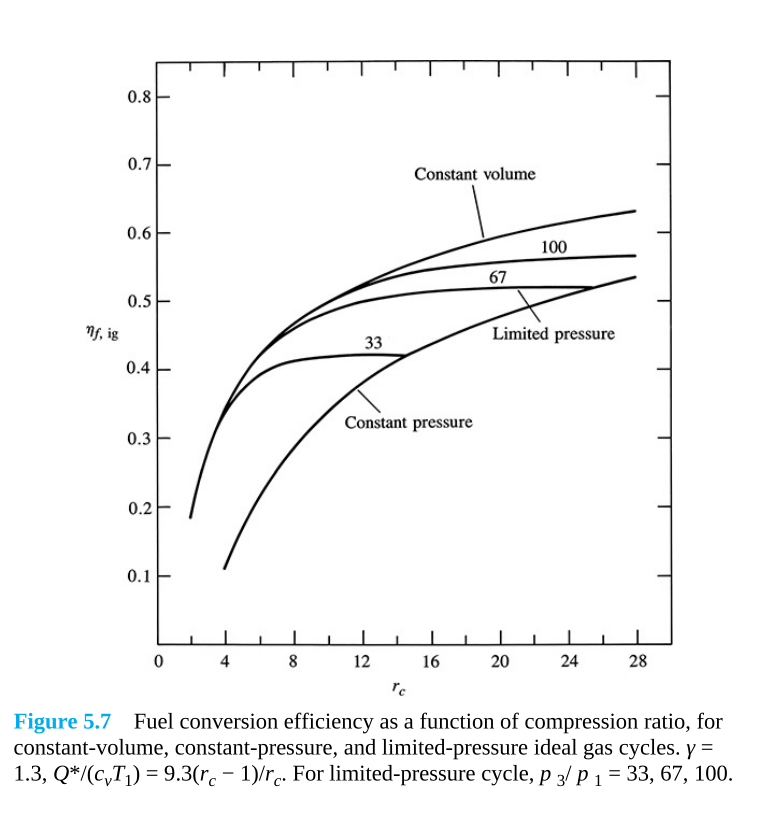
\includegraphics[width=.7\textwidth]{rendimiento_conv_comb.png}
    \caption{Rendimiento de conversión de combustible en función de $r_c$ para
    ciclos de gas ideal de volumen constante, presión constante y presión
    limitada(cambiar por propia??)} \label{fig:rendimientos}
    %
\end{figure}

Uno de los aspectos atractivos del MRCVC es la combustión a volumen consatante,
la cual ocurre por la geometría de la cámara de combustión, en la figura
\ref{fig:ciclo_mrcvc} se presenta el diagrama $P-V$ de una simulación de ICESym
del MRCVC.
%
\begin{figure} \centering
    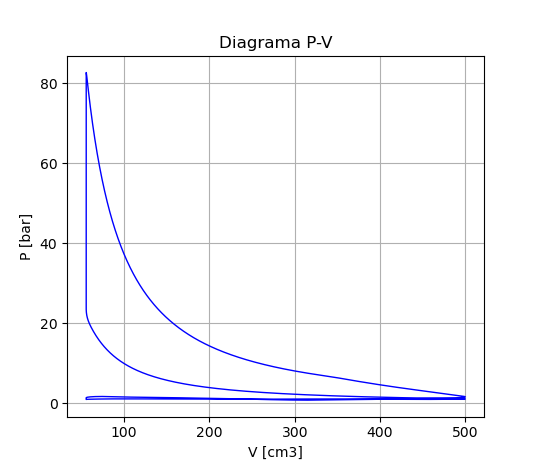
\includegraphics[width=.7\textwidth]{ciclo/diagramaPV.png}
    \caption{Diagrama P-V del MRCVC}\label{fig:ciclo_mrcvc}
    %
\end{figure}


\subsection{Motores rotativos}
%
Los motores rotativos son una variable al diseño más popular de los motores
alternativos, su compacidad, balanceo y mayores velocidades de giro los vuelven
más atractivos en aplicaciones en las cuales el volumen es restringido.
%
La mayor velocidad de giro permite alcanzar mayores potencias por lo que tiene
una menor relación peso/potencia que motores reciprocantes de potencia similar.
%
El motor rotativo más conocido es el Wankel, cuyo primer prototipo funcional se
desarrolló cerca del 1957. 
%
En la actualidad se cuenta con otros desarrollos de este tipo de motores como
el motor rotativo de pistón líquido, con un ciclo de combustión a volumen
constante denominado HECH\parencite{hehc_05}, similar al del MRCVC.

Si bien son una alternativa interesante a los motores reciprocantes, estos
motores requieren introducir aceite en la cámara de combustión para lubricar
las partes móviles, además tienen una mayor superficie de transferencia de
calor por lo que la pérdida de calor es mayor en comparación con los
reciprocantes.
%
En la actualidad, los requisitos de niveles de emisiones ambientales de ciertos
gases hacen de estos motores inviables para el uso comercial, sin embargo la
compacidad del motor los vuelve atractivos en aplicaciones militares como por
ejemplo para vehículos aéreos no tripulados.

%%%%%%%%%%%%%%%%%%%%%%%%%%%%%%%%%%%%%%%%%%%%%%%%%%%%%%%%%%%%%%%%%%%%%%%%%%%%%%%

\subsection{Parámetros Operativos e Indicadores de rendimiento}
%
En esta sección se describen brevemente los parámetros operativos e indicadores
de rendimiento en general y los utilizados en este trabajo en particular.
%
Algunas de las características más importantes de un motor son:
%
\begin{enumerate}
        %
    \item Potencia máxima
        %
    \item Torque máximo
        %
    \item Rango de velocidades de operación
        %
    \item Consumo de combustible, costo del combustible
        %
    \item Costo inicial, de operación, de mantenimiento, ...
        %
    \item Confiabilidad
        %
    \item Ruido y emisiones contaminantes
        %
\end{enumerate}

Estos aspectos permiten al usuario final  comparar entre diferentes
alternativas de motores para decidir cuál es el que mejor aplica a la función
que se le quiere dar.
%
Se pueden expresar de manera más concreta con algunos parámetros geométricos e
indicadores de rendimiento particulares a la geometría de cada motor o
adimensionalizados por características geométricas, por ejemplo algunas
características se pueden relacionar con el volumen desplazado (también
conocido como cilindrada) para permitir la comparación entre diferentes
geometrías.

%%%%%%%%%%%%%%%%%%%%%%%%%%%%%%%%%%%%%%%%%%%%%%%%%%%%%%%%%%%%%%%%%%%%%%%%%%%%%%%

\subsubsection{Volumen Desplazado}
%
El volumen desplazado se define como la diferencia entre el volumen máximo y
mínimo que ocupa la cámara de combustión.

\begin{equation}\label{eq:vol_desp}
    V_d = V_{max}-V_{min}
\end{equation}

% La geometría de la càmara de combustión del MRCVC está definida por leyeEn el
% MRCVC la geomeria de la cámara de combustión es m'0

%%%%%%%%%%%%%%%%%%%%%%%%%%%%%%%%%%%%%%%%%%%%%%%%%%%%%%%%%%%%%%%%%%%%%%%%%%%%%%%

\subsubsection{Relación de compresión}

Se define como el cociente ente el volumen máximo y el volumen mínimo del
ciclo, es uno de los parámetros más importantes de un motor, ya que afecta la
presión máxima que se puede obtener en la cámara, esto afecta la
\emph{performance}, potencia entregada, esfuerzos mecánicos y rendimiento del
motor.

\begin{equation}\label{eq:rel_comp}
    r_c = \frac{V_{max}}{V_{min}} = \frac{V_d+V_c}{V_c}
\end{equation}

%%%%%%%%%%%%%%%%%%%%%%%%%%%%%%%%%%%%%%%%%%%%%%%%%%%%%%%%%%%%%%%%%%%%%%%%%%%%%%%

% \subsubsection{Troque y potencia al freno}
% NOTA: Hace flata?

%%%%%%%%%%%%%%%%%%%%%%%%%%%%%%%%%%%%%%%%%%%%%%%%%%%%%%%%%%%%%%%%%%%%%%%%%%%%%%%

\subsubsection{Trabajo indicado por ciclo}
%
El trabajo entregado por ciclo de operación se denomina trabajo indicado por
ciclo y se obtiene de integrar la curva del diagrama P-V del motor.

\begin{equation}\label{eq:w_indicado}
    W_{c,i} = \oint P dV
\end{equation}

De esta curva se debe diferenciar entre trabajo bruto y trabajo neto, en el
último se tiene en cuenta el trabajo de bombeo, que resulta de la diferencia
del trabajo realizado durante las carreras de admisión y escape, por lo que
este indicador se puede diferenciar en trabajo bruto indicado por ciclo
$W_{c,ig}$, trabajo neto $W_{c_in}$ indicado por ciclo y la diferencia entre
ambas es el trabajo de bombeo $W_{bombeo}$.
%
El valor de $W_{c,ig}$ mide el trabajo realizado por el motor en las carreras
de compresión y expansión.
%
$W_{c,in}$ mide el trabajo realizado por el motor considerando las 4 carreras
del ciclo.

%%%%%%%%%%%%%%%%%%%%%%%%%%%%%%%%%%%%%%%%%%%%%%%%%%%%%%%%%%%%%%%%%%%%%%%%%%%%%%%

% \subsubsection{Rendimiento Mecánico}

%%%%%%%%%%%%%%%%%%%%%%%%%%%%%%%%%%%%%%%%%%%%%%%%%%%%%%%%%%%%%%%%%%%%%%%%%%%%%%%

\subsubsection{Consumo especifico de combustible y eficiencia de conversión de
combustible}
%
El consumo especifico de combustible \emph{sfc}, se define como el caudal
másico de combustible ($\dot{m_f}$) por unidad de potencia $P$ entregada por el
motor.

\begin{equation}\label{eq:sfc}
    sfc = \frac{\dot{m_f}}{P}
\end{equation}

Este indicador mide la eficiencia con la que el motor utiliza el combustible
para una condición de operación dada, para motores de encendido por chispa se
tienen valores típicos para de alrededor de $65\mu g/J$.

Una versión similar de este indicador, pero adimensionalizada en relación a la
energía suministrada por el combustible, es la \emph{eficiencia de conversión
de combustible} $\eta_f$, que se relaciona al \emph{sfc} por medio del poder
calórico del combustible, $Q_{HV}$.

\begin{equation}\label{eq:eta_f}
    \eta_f = \frac{1}{sfc \cdot Q_{HV}}
\end{equation}

El valor de $Q_{HV}$ es una propiedad del combustible y se determina en un
ensayo de laboratorio, valores típicos para los combustible comerciales
basados en hidrocarburos son 42 a 44 $MJ/kg$

%%%%%%%%%%%%%%%%%%%%%%%%%%%%%%%%%%%%%%%%%%%%%%%%%%%%%%%%%%%%%%%%%%%%%%%%%%%%%%%

\subsection{Presión Media Efectiva}
%
La presión media efectiva o $mep$ por sus siglas en inglés, es una medida
similar al torque pero adimensionalizada por el tamaño de cada motor.
%
El trabajo realizado por ciclo se puede calcular como $W_c = \frac{P \cdot
n_r}{N}$, donde $n_R$ es el número de revoluciones del cigüeñal por cada
carrera de expansión por cilindro.
%
Para motores de cuatro tiempos $n_R=2$ y $n_R=1$ para motores de dos tiempos.

La presión media efectiva se define como:

\begin{equation}\label{eq:mep}
    mep = \frac{P \cdot n_R}{V_d \cdot N}
\end{equation}

Se puede diferenciar entre presión media efectiva indicada (\emph{imep}), al
freno (\emph{bemp}) y de fricción (\emph{fmep}), utilizando el valor de
potencia correspondiente en la ecuación \ref{eq:mep}.
%
El valor de \emph{mep} (al igual que el torque) de un motor varía con la
velocidad de operación, siguiendo de cerca la curva de rendimiento volumétrico
como se puede ver en la figura \ref{fig:bmep_tipica}.

En la actualidad, motores SI naturalmente aspirados tiene valores de
\emph{bmep} de entre 1050 a 1250 kPa para la velocidad a la que se alcanza el
mayor torque.

\begin{figure}
    \centering
    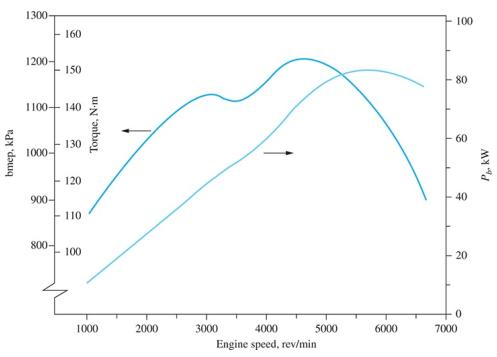
\includegraphics[width=0.7\textwidth]{curva_bmep_tipica.jpg}
    \caption{\emph{bmep}, torque y potencia vs velocidad de operación\parencite{heywood}.}
    \label{fig:bmep_tipica}
\end{figure}

%%%%%%%%%%%%%%%%%%%%%%%%%%%%%%%%%%%%%%%%%%%%%%%%%%%%%%%%%%%%%%%%%%%%%%%%%%%%%%%

\subsection{Rendimiento Volumétrico}
%
El rendimiento volumétrico mide la eficiencia del sistema de admisión y se
define como el cociente entre el caudal másico de aire que ingresa al sistema
de admisión y la velocidad con la que el volumen es desplazado por el pistón
combustión.

\begin{equation}\label{eq:eta_v}
    \eta_v = \frac{2\dot{m_a}}{\rho_{a,i}V_d N} = \frac{m_a}{\rho_{a,i}V_d}
\end{equation}

Para motores naturalmente aspirados, la densidad del aire de admisión
$\rho_{a,i}$ se toma comúnmente como la densidad atmosférica por lo que
$\eta_v$ mide el rendimiento de todo el sistema de admisión.

El valor de rendimiento volumétrico máximo para motores naturalmente aspirados
ronda el 90\%, hay varios fenómenos que afectan al rendimiento volumétrico,
entre los más importantes están:

\begin{itemize}
    %
    \item Efectos cuasiestáticos: combustible, relación aire/combustible,
        vaporización del combustible en el conducto de admisión, temperatura
        del aire de admisión, relación entre presión de admisión y escape,
        relación de compresión, etc.
    %
    \item Pérdidas de carga por fricción viscosa. 
    %
    \item Pérdidas de carga localizada.
        %
        Los elementos del sistema de admisión causan caídas de presión.
    %
    \item Transferencia de calor en sistema de admisión.
        %
        La mezcla se calienta por transferencia de calor, lo que disminuye la
        densidad de la misma, reduciendo la masa disponible para la cámara de
        combustión.
    %
    \item Reglaje de las válvulas/puertos.
        %
        El punto de apertura y cierre de los puertos (puesta a punto o reglaje)
        es clave para el funcionamiento del motor, dependiendo de la puesta a
        punto se verá favorecido el flujo a determinada velocidad de operación.
    %
    \item Flujo bloqueado en puertos de admisión y escape.
        %
        En las zonas de menor área de pasaje, la velocidad del fluido puede
        aumentar hasta alcanzar la velocidad del sonido, esto se conoce como
        bloqueo y limita el caudal másico que puede ingresar a la cámara de
        combustión. 
    %
    \item Transferencia de calor en el cilindro.
        %
        La cámara de combustión se encuentra a mayor temperatura que la mezcla
        que ingresa, esto hace que aumente la el volumen específico ,
        reduciendo la cantidad que puede ingresar.
    %
    \item Sintonía del puerto de admisión y escape.
        %
        El diseño de los puertos de admisión y escape puede favorecer el
        funcionamiento de los mismos a determinada velocidad de operación, esto
        se logra aprovechando las ondas de presión que se producen por la
        apertura y cierre de las válvulas.
        %
    \item Sobrecarga.
        %
        Por medio de un compresor o turbocompresor se aumenta la presión en el
        sistema de admisión, forzando más aire a la cámara de combustión.
    %
    \item Efecto RAM.
        %
        A grandes velocidades de flujo, la inercia del gas produce un aumento
        de presión al momento del cierre del puerto de admisión, esto causado
        por restricción que se genera. Una sobrepresión en el puerto de
        admisión permite un mayor flujo másico al cierre del puerto de
        admisión.
        %
\end{itemize}

La curva de rendimiento volumétrico es muy similar a la curva de torque o de
presión media efectiva, esto es así porque indica la cantidad de masa de aire
que ingresa al cilindro (o de mezcla aire-combustible) y es esta masa la que
limita el total del trabajo que se puede producir.
%
Esto se ve claramente en un motor de inyección directa, donde la cantidad de
combustible a inyectar está limitada por la masa de aire sin quemar en la
cámara de combustión para mantener la relación de aire combustible con la que
opere de manera estable el motor.


Este indicador es central en este trabajo y se buscó que el software
desarrollado devuelva un espectro de opciones de configuración de los puertos,
de los cuales se pueda seleccionar la mejor geometría teniendo en cuenta el
efecto sobre el rendimiento volumétrico.
%
Analizar detalladamente los efectos que hacen al valor final de $\eta_v$ es de
una complejidad que excede a este trabajo, en su lugar se buscó maximizar
$\eta_v$ sin entrar en detalle de los efectos presentes.
%
Se buscó una curva de rendimiento volumétrico con un máximo para altas
revoluciones de modo de aprovechar el balanceo del motor para maximizar el trabajo
realizado a altas velocidades para obtener potencias altas a altas RPM, a su vez
se buscó mantener valores de fracción de gases residuales $x_r$ relativamente
bajas..
%
Estos efectos se describen en detalle en la literatura\parencite{heywood}, para
este trabajo se tiene las siguientes consideraciones: 

\begin{enumerate}
        %
    \item El combustible utilizado es isooctano, la mezcla aire-combustible es
        estequeométrica ($\phi=1$).
        %
    \item El sistema de intercambio de gases del MRCVC se compone de un
        conducto y puerto admisión, conducto y puerto de escape.
        %
    \item Los conductos se asumen como elementos rectos de un largo finito y
        diámetro constante, cuya fuente y sumidero es la atmósfera a $101330.0
        Pa$ y $25^{\circ}C$.
        %
    \item La temperatura de la pared de la cámara de combustión se asume en
        450K.
        %
    \item El motor es naturalmente aspirado.
        %
\end{enumerate}

%%%%%%%%%%%%%%%%%%%%%%%%%%%%%%%%%%%%%%%%%%%%%%%%%%%%%%%%%%%%%%%%%%%%%%%%%%%%%%%

\subsubsection{Sincronización del sistema de admisión}
%
% Al abrir el puerto de admisión se pone en contacto los gases residuales de la
% cámara de combustión con la masa fresca en el puerto de admisión, estos dos
% volúmenes se encuentran a diferente presión que tiende que tiende a 
%
En motores naturalmente aspirados, al momento de abrir la válvula o puerto de
admisión, los gases residuales en la cámara se encuentran a una presión mayor
que la masa fresca en el puerto de admisión, esta diferencia de presión produce
una onda de depresión que viaja desde la cámara de combustión hacia el extremo
opuesto del conducto de admisión.
%
Cuando esta onda de presión llega al plenum de admisión, se refleja como una
onda de sobrepresíon que toma un tiempo $t$ en alcanzar nuevamente el puerto,
si el tiempo que toma la onda en reflejarse es tal que alcanza la válvula justo
antes del cierre de la misma se dice que el puerto el sistema está sintonizado.
%
Esta sopbrepresión permite que ingrese una mayor cantidad de masa fresca a la
cámara de combustión, aumentando la cantidad de trabajo que se puede realizar.

En la figura\ref{fig:sintonia1} se muestra el diagrama de presión vs ángulo de
cigüeñal para 1200 y 4800 RPM, en donde se indican los períodos en los que se
encuentran abiertos las válvulas de admisión (IO) y de escape (EO).
%
Los valores $p_1$, $p_2$ y $p_3$ hacen referencia diferentes longitudes de los
conductos de admisión y escape.
%
Se puede ver que para $p_1$ a 4800 RPM hay un claro pico de presión justo al
cierre del puerto de admisión, con esto el puerto está sintonizado para esta
velocidad.

\begin{figure}
    \centering
    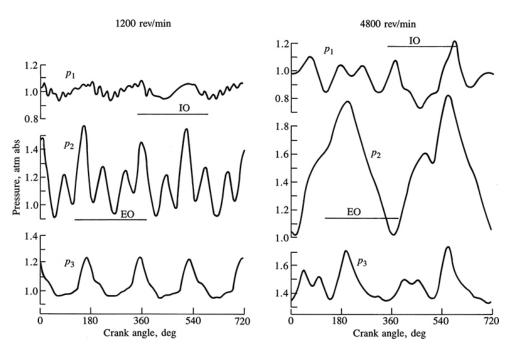
\includegraphics[width=0.7\textwidth]{sintonia_heywood.jpg}
    \caption{(cambiar por una del mrcvc) Diagrama de presión vs ángulo de cigüeñal}\label{fig:sintonia1}
\end{figure}

Debido a que la onda de presión debe viajar dos veces longitud del conducto de
admisión desde el momento que abre el puerto de admisión, para sincronizar el
sistema de admisión a bajas velocidades, se requieren longitudes mayores lo que
hace más grande el sistema de admisión.
%
La sincronía a mayores velocidades de admisión es preferida, porque usualmente
se tiene el máximo de torque y de potencia a mayores RPM, además reduce la
necesidad de conductos mámás largos.
%
En motores multi cilíndricos se utiliza un plenum de admisión, este dispositivo
proporciona un volumen grande de aire que se utiliza como resonador.
%
Se puede hacer vibrar de modo que las oscilaciones de presión internas envían
ondas de sobre presión a cada puerto en el momento preciso en el que se
aproxima el cierre del mismo.

%%%%%%%%%%%%%%%%%%%%%%%%%%%%%%%%%%%%%%%%%%%%%%%%%%%%%%%%%%%%%%%%%%%%%%%%%%%%%%%

\subsubsection{Sincronización del sistema de escape}

De forma análoga al puerto de admisión, al momento de la apertura del puerto o
válvula de escape los gases residuales de la combustión se encuentran a una
mayor presión que el gas en el conducto, esto crea una onda de sobrepresión que
viaja por el escape hasta alcanzar el final del mismo o un área de gran
volumen, como el catalizador o el silenciador.
%
Desde esta zona se refleja como una onda de depresión, que si alcanza el puerto
justo antes del cierre del mismo ayuda a evacuar una mayor cantidad de gas,
disminuyendo la cantidad de gases residuales presentes para el próximo ciclo.

Reducir la cantidad de gases residuales tiene dos efectos beneficiosos, en
primer lugar estos gases ocupan volumen en la cámara de combustión, además
porque su elevada temperatura (en relación a la masa fresca) calienta el gas
que ingresa al cilindro desde el puerto de admisión, aumentando el volumen
específico y reduciendo el rendimiento volumétrico.

En la figura \ref{fig:sintonia1} se ve que para el escape en $p_2$ se tiene una
depresión justo al cierre del puerto, este sistema está sintonizado para 4800
RPM, es notorio el contrate con el mismo puerto a 1200 RPM, en donde se ve un
pico de presión cerca del cierre del puerto.

%%%%%%%%%%%%%%%%%%%%%%%%%%%%%%%%%%%%%%%%%%%%%%%%%%%%%%%%%%%%%%%%%%%%%%%%%%%%%%%

\subsubsection{Fracción de gases residuales}
%
La fracción de gases residuales $x_r$ mide la cantidad de gases quemados que
hay en el cilindro al inicio de la carrera de admisión.
%
Esto ocurre principalmente por dos razones, en primer lugar queda gas atrapado
en el cilindro, remanente del ciclo anterior y en segundo lugar puede existir
un reflujo desde el puerto de escape hacia la cámara de combustión si hay
solape de válvulas, lo que afecta: rendimiento volumétrico, trabajo obtenido,
eficiencia y emisiones.

En el MRCVC existe además solape de cámara, este es un fenómeno en el que una
cámara en proceso de admitir gases frescos se ve afectada por la apertura del
puerto de admisión a la cámara siguiente, que se encuentra a mayor presión y
temperatura por estar culminando el proceso de escape y comenzando el de
admisión, esto reduce el rendimiento volumétrico.
%
% Un esquema de este proceso se puede ver en la figura \ref{fig:reflujo_solape}.
% falta la figura
